\documentclass[a4paper, titlepage]{article}

\usepackage{microtype}
\usepackage{amsmath}
\usepackage{index}
\usepackage{fancyhdr}
\usepackage[hidelinks]{hyperref}
\usepackage{float}
\usepackage{tabularx}
\usepackage{tikz}
\usepackage{graphicx}
\usepackage{ltablex}
\usepackage[left=4cm,right=4cm]{geometry}
\usepackage{subcaption}
\usepackage{listings}

\hypersetup{
	colorlinks=true,
	linktoc=all,    
	linkcolor=black,
	%linktocpage
}

\usetikzlibrary{positioning, shapes, calc}

\renewcommand{\lstlistingname}{Algorithm}% Listing -> Algorithm

\begin{document}

\title{}
\author{Alex Greig}
\begin{titlepage}
	\centering
	
\includegraphics[width=0.5\textwidth]{sta-logo.png}\par
	\vspace{1.5cm}
	\noindent\rule{12cm}{0.07cm} \\
	\vspace{0.2cm}
	{\huge{\textbf{Nodepaths\\Design Documentation - Task 2}}\\}
	\vspace{0.2cm}
	\noindent\rule{12cm}{0.07cm} \\
	\vspace{1.5cm}
	{\LARGE{\emph{By Alex Greig}}} \\
	\vspace{1.5cm}
	{\large{\emph{ \today}}}
	\vfill
\end{titlepage}

\tableofcontents
\vfill
\section{Project Portfolio}

\subsection{Problem Definition}
The problem with today's internet is the control large corporations have over information transmission, enabling data to be lost, monetized, or given to the government, all without users knowing. Another problem of the internet is the inherent security flaws associated with centralised control; that is, its ability to be hacked. The final problem is the inequality of the internet as large populations throughout the world are unable to access the internet, with access they would be able to receive better educational resources, progressing humanity forward. \\


The application that I am creating is called Nodepaths, and it is important for the consumer market as it will provide high security to user's data and a network that is robust and resistant to problems allowing for secure data transfer between devices globally, solving the problems above. The application will have a significant effect on the way we use the internet and allow users to share, communicate and complete complex computational tasks efficiently and securely. The application will be a decentralised network that uses peer-to-peer architecture and mesh topology, allowing any machine capable of connecting to a network to join and become a "node". The application will also include the feature of Wi-Fi peer to peer transmission allowing for nodes to be connected by Wi-Fi radio waves eliminating costs of telecommunication services, however, if users cannot be connected by the mesh then cellular internet is available. This information will be encrypted, end to end. The mesh network will relay data and messages using a wireless ad-hoc network, where data is propagated along a path by hopping from node to node until it reaches its destination. The paths will be calculated based on the Ad-Hoc On Demand Vector Routing protocol (AODV), a routing protocol that determines and maintains routes whenever they are required. \\

The application that I am creating, Nodepaths, will have three main functions. The first is creating a user, to do this it will need to create identification. The application will create a public and private key using the Curve25519 elliptic curve in conjunction with the Diffie–Hellman key agreement scheme and the Advanced Encryption Standard, then a psuedo-random IPv4 Address and finally validate a username that has been entered by the user. The second function of Nodepaths is to transfer data, normally messages, over a wireless ad-hoc network to another node. The final main function of the application will be to give users the ability to add new nodes (friends) to the application allowing them to select friends that they want to text to. These three functions when integrated will provide the foundation for a user-friendly text messaging application that runs on a decentralised, distributed network. Although the functions may seem simple or basic the underlying backend behind a network of this caliber is complex; to function, innovative solutions are needed. \\

Future improvements and upgrades to the application will include the implementation of Blockchain technology to provide digital transactions and a cryptographic wallet on the application, eliminating the need for banks and other financial institutions. In the future, the application may also provide assistance to disadvantaged communities as it would give them communication without the cost of telecommunication services.

\subsection{Context and Data-flow Diagrams}
\vspace{2cm}
\begin{figure}[H]
\caption{Context Diagram}
\vspace{1cm}
\centering
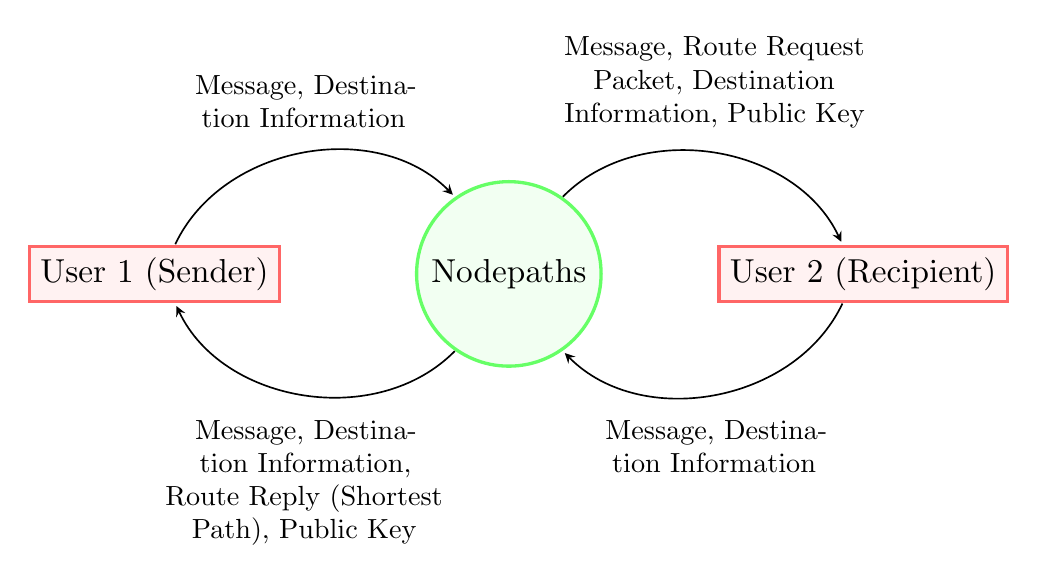
\begin{tikzpicture}[
roundnode/.style={circle, scale = 1.2, draw=green!60, fill=green!5, very thick, minimum size=7mm},
squarednode/.style={rectangle, scale = 1.2, draw=red!60, fill=red!5, very thick, minimum size=5mm},
to/.style={->,>=stealth,shorten >=1pt,semithick},
]
%nodes
\node[squarednode](e1) at (-4.5, 0) {User 1 (Sender) };
\node[roundnode](p) at (0,0) {Nodepaths};
\node[squarednode](e2) at (4.5, 0) {User 2 (Recipient)};
%connections
\draw[to] (e1) to [bend left = 55] node[align=center, text width = 4cm, above = 0.2cm] {Message, Destination Information}(p);
\draw[to] (p) to [bend left = 55] node[align=center,text width = 4cm, midway, below = 0.2cm] {Message, Destination Information, Route Reply (Shortest Path), Public Key}(e1);
\draw[to] (p) to [bend left = 55] node[align=center,text width = 4cm, midway, above = 0.2cm] {Message, Route Request Packet, Destination Information, Public Key}(e2);
\draw[to] (e2) to [bend left = 55] node[align=center,text width = 4cm, midway, below = 0.2cm] {Message, Destination Information}(p);
\end{tikzpicture}
\end{figure}

\begin{figure}[H]
\caption{Data Flow Diagram}
\vspace{1cm}
\centering
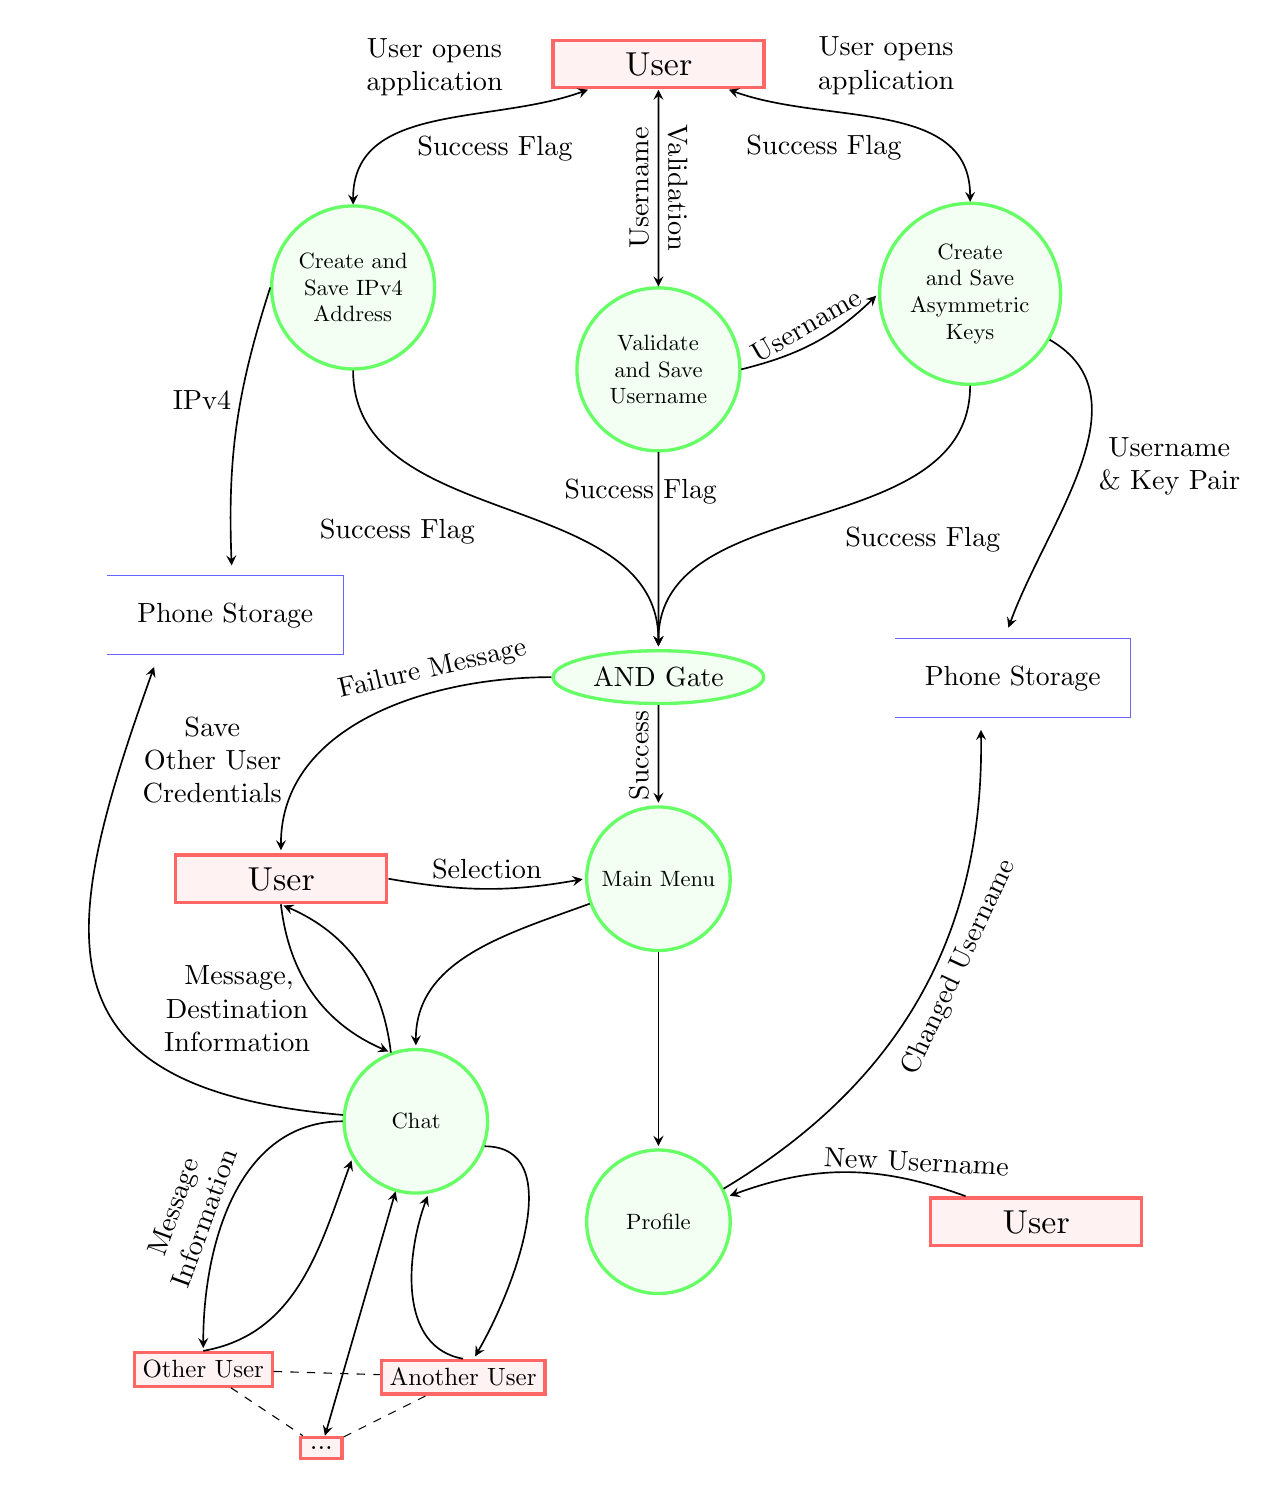
\begin{tikzpicture}[node distance = 2.5cm,
process/.style={circle, scale = 0.8, align=center, text width = 2cm, draw=green!60, fill=green!5, very thick, minimum size=7mm},
entity/.style={rectangle, scale = 1.2, align=center, text width = 2cm, draw=red!60, fill=red!5, very thick, minimum size=5mm},
path/.style={->,>=stealth,shorten >=1pt,semithick},
]

\tikzset{
  pics/datastore/.style args={#1,#2, #3}{
     code={
	     \draw [draw=blue!60] (0,0) -- (3,0) -- (3,1) -- (0, 1);
	     \node[#3] (#1) at (1.5,0.5) {#2};
     }
  }
}

%Nodes
\node [entity] (user) {User};
\node [process] (c_ip) [below left = of user]{Create and Save IPv4 Address};
\node [process] (c_ak) [below right = of user]{Create and Save Asymmetric Keys};
\node [process] (s_username) [below = of user]{Validate and Save Username};
\node [draw, ellipse, draw=green!60, fill=green!5, very thick] (and) [below = of s_username] {AND Gate};
\draw (3, -8.3) pic{datastore={pstore, Phone Storage, black}};
\draw (-7, -7.5) pic{datastore={pstore2, Phone Storage, black}};
\node [process, yshift=-3.2cm] (m_menu) at (and) {Main Menu};
\node [entity] (user2) [left = of m_menu] {User};
\node [process] (chat) [below left = of m_menu] {Chat};
\node [process] (profile)  [below = of m_menu] {Profile};
\node [scale =0.9, yshift = -3.5cm, xshift = -3cm, align=center, draw=red!60, fill=red!5, very thick] (u1) at (chat) {Other User};
\node [scale = 1, yshift = -1cm, xshift = 1.5cm, align=center, draw=red!60, fill=red!5, very thick] (u2) at (u1) {...};
\node [scale =0.9, yshift = 1 cm, xshift = 2cm, align=center, draw=red!60, fill=red!5, very thick] (u3) at (u2) {Another User};
\node [entity] (user3) [right = of profile] {User};

% Paths

\draw [stealth-stealth, semithick](user) edge[out=200, in=90] node[align=center, midway, text width=2.5cm, above = 0.2cm] {User opens application} node[align=center, pos=0.3, text width=2.5cm, below = 0.2cm] {Success Flag} (c_ip); 
\draw [stealth-stealth, semithick] (user) to node[align=center, text width=2.5cm, midway, rotate = 90, above] {Username} node[align=center, text width=2.5cm, midway, rotate = 270, above] {Validation} (s_username); 
\draw [stealth-stealth, semithick](user) edge[out=340, in=90] node[align=center, midway, text width=2.5cm, above = 0.2cm] {User opens application} node[align=center, pos=0.3, text width=2.5cm, below= 0.2cm] {Success Flag} (c_ak); 

\draw (c_ip) edge[out=270, in=90, path] node[align=center, midway, text width=2.5cm, below left] {Success Flag}(and);
\draw (c_ak) edge[out=270, in=90, path] node[align=center, midway, text width=2.5cm, below right] {Success Flag}(and);
\draw [path] (s_username) to node[align=center, pos=0.2, xshift=-2.25mm] {Success Flag} (and); 
\draw [path] (and) to node[align=center, midway, rotate=90, above] {Success} (m_menu); 
\draw (and) edge[out=180, in=90, path] node[align=center, pos=0.3, above, rotate=13] {Failure Message} (user2);
\draw [path] (user2.0) to [bend right = 10] node[align=center, text width = 4cm, midway, above] {Selection} (m_menu.west);

\draw (m_menu) edge[out=200, in=90, path] (chat); 
\draw [path] (m_menu) to (profile); 
\draw [path] (user2.south) to [bend right = 30] node[align=center, pos=0.6, left, text width = 2cm] {Message, Destination Information} (chat.110);
\draw [path] (chat.110) to [bend right = 30] (user2.270);

\draw (chat) edge[out=180, in=90, path] node[align=center, pos=0.6, text width = 2cm, rotate=70, above] {Message Information} (u1);
\draw (u1.north) edge[out=10, in=250, path] (chat.210);
\draw (chat.-20) edge[out=0, in=60, path] (u3);
\draw (u3.north) edge[out=170, in=250, path] (chat.280);
\draw [dashed](u1) -- (u2);
\draw [dashed](u2) -- (u3);
\draw [dashed](u1) -- (u3);
\draw [stealth-stealth, semithick](u2) -- (chat);

\draw [path] (user3) to [bend right = 20] node[align=center, pos=0.2, above, text width = 3cm, rotate=-3] {New Username} (profile);

\draw [path] (c_ip.west) to [bend right = 10] node[align=center, pos=0.4, xshift=-0.5cm, text width = 3cm] {IPv4} ($(c_ip.west)!3.6cm!(pstore2)$);
\draw [path] (s_username.east) to [bend right = 15] node[align=center, pos=0.5, above, text width = 2cm, rotate=30] {Username} (c_ak.west);
\draw [path] (c_ak) edge[out=330, in=70] node[align=center, pos=0.5, right, text width = 2cm] {Username \& Key Pair} ($(c_ak)!4.3cm!(pstore)$);
\draw [path] (profile) to [bend right = 30] node[align=center, rotate=65, pos=0.58, below]{Changed Username}($(profile)!7.5cm!(pstore)$);
\draw [path, shorten >= 0.4cm] (chat) .. controls (-8, -13) and (-7.6, -11) .. node[align=center, pos=0.85, right, text width = 2cm] {Save Other User Credentials} (pstore2.200);
\end{tikzpicture}
\end{figure}

\subsection{Structure Chart}

\subsection{Algorithms}

\renewcommand{\ttdefault}{pcr}
\lstset{
	basicstyle=\small\ttfamily,
	captionpos=t,
	numbers=left,
	tabsize=4,
	keywordstyle=\bfseries,
	breaklines=true,
	columns=fullflexible,
	numbersep=-8pt, 
	frame = shadowbox,
	morekeywords={BEGIN, END, DISPLAY, INPUT, IF, ENDIF, WHILE, DO, ELSE, THEN, OR, OPEN, RETURN, WRITE, NEXT, FOR, APPEND, CLOSE, PASS, AND, OUTPUT}
}

The core algorithms that will be used in the application are displayed below, written in the pseudocode syntax:

\begin{lstlisting}[caption=Main Program, escapechar=\@]
	BEGIN MAINPROGRAM
		username, keys, ipv4 = @\underline{LoadNode()}@
		DISPLAY "Enter another Node's Username to Message or type Quit to Exit"
		INPUT Selection
		WHILE Selection <> "Quit" DO
			Display "Please Input your message: "
			Input Message 	
			Reply = SendMessage(Message, TargetUser, Reply, keys[1]) //keys[1] is the secret key
			Display Reply
			DISPLAY "Enter another Node's Username to Message or type Quit to Exit"
			INPUT Selection
		END WHILE
	END MAINPROGRAM
\end{lstlisting}

The main program above displays different processes, inputs and outputs that would be in the real program, however, this code isn't a full replication of the intended end product. If I was to create this application in full I would have more functions that separate the program into smaller pieces, making it easier to read and write. The first difference from the code above is I would separate all the screens into different functions however as previously mentioned this is impractical for the intention of the task.

\begin{lstlisting}[caption=Load Node, escapechar=\@]
	BEGIN  @\underline{LoadNode(username, keys, ipv4)}@
		username = ""
		keys = a fixed size array of allowing two byte arrays of length, 32 // [[u8; 32]; 2]
		ipv4 = ""
		OPEN "Phone Storage" for INPUT and OUTPUT
			// Checking if config file exists, False if user is opening for the first time.
			IF "PhoneStorage/config.toml".exists() == True DO
				lines = READ lines from "Phone Storage/config.toml" into an array
				//Below is cycling throught the node config file and loading the values into the program from storage
				username = lines[0]
				keys = lines[1].split[","]
				ipv4 = lines[2]

			ELSE DO
				CreateFile("PhoneStorage/config.toml")
				INPUT unvalidated_username
				//Validates Length
				success = False
				WHILE success == False DO
					IF unvalidated_username.len() >= 5 OR unvalidated_username.len() <= 20 THEN
						success = True
						username = unvalidated_username
					ENDIF
				END WHILE
				ipv4 = @\underline{CreateIPv4()}@
				keys = @\underline{CreateEccKeys(secretKey, publicKey)}@
			END IF
			WRITE username, ipv4, keys
		CLOSE "Phone Storage"
		RETURN username, keys, ipv4
	END  @\underline{LoadNode}@
\end{lstlisting}

\begin{lstlisting}[caption=Elliptic-Curve Cryptographic (ECC) Key Generation, escapechar=\@]
	BEGIN  @\underline{CreateECCKeys(secretKey, publicKey}@

		curve = get_curve('curve25519')
		k = rand_num(0, 627710173538668) //Parameters is the starting and ending range of the random number
		secretKey = k
		publicKey = privKey * curve.basepoint 

		RETURN secretKey, publicKey
	END  @\underline{CreateECCKeys}@
			
\end{lstlisting}
The Elliptic-Curve Cryptographic Algorithm is efficient and as fast as simply creating a random number, however, it allows for a private and public key to be created. The algorithm itself is based on an elliptic curve which are created through the equation: \[ y^2 = x^3 + ax + b \] Due to this equation given a curve which has infinite points, we will limit the curve to a finite field. To do this we use modular arithmetic which transforms the equation into the form: \[ y^2 = x^3 + ax + b(mod\ p)\] where p is a prime number between $3$ and $2^{256}$. This is a general equation for an elliptic graph however certain specific equations have been named such as secp256k1 (used in Bitcoin), which is \[y^2 = x^3 + 7 (mod\ 17) \] To check whether a point, for example $P(3,4)$, lies on this curve you substitute values in to x and y in the equation. A point G over an elliptic curve can be multiplied by an integer k and the result is another EC point P on the same curve and this operation is fast. This is the basis behind the key generation, we multiply a fixed EC point G (the generator point or base point) by certain integer k (k can be considered as private key), we obtain an EC point P (its corresponding public key). It is very fast to calculate $P = k * G$ and extremely slow (considered infeasible for large k) to calculate $k = \frac{P}{G}$.

\begin{lstlisting}[caption= IPv4 Creation, escapechar=\@]
	BEGIN  @\underline{IPv4Gen(ip)}@

	ip = "192.168"
	FOR i = 0 to 1 DO
		APPEND random_int(0, 255) to base_ip
	NEXT i
	END FOR
	RETURN ip	
	END  @\underline{IPv4Gen}@
\end{lstlisting}

\begin{lstlisting}[caption=Send Data Packets over Network, escapechar=\@]
	BEGIN  @\underline{SendMessage(Message, User, Reply, secretKey)}@
		transmitter = WifiPeertoPeerApi()
		transmitter.perform_handshake(User)
		transmitter.send_udp_packet(RREQ, User) //finding the shortest path to the designated user
		timeout_time = 10
		path = transmitter.reply(timeout_time)
		transmitter.send_udp_packet(Request_Public_Key, User, path)
		their_public_key = transmitter.reply(timeout_time)
		shared_secret_key = diffie_hellman(secretKey, their_public_key)
		encrypted_message = encrypt(Message, shared_secret_key)
		transmitter.send_udp_packet(Message, User, path)
		encrypted_reply = transmitter.reply(timeout_time)
		Reply = decrypt(encrypted_reply, shared_secret_key)
		RETURN Reply
	END  @\underline{SendMessage}@
			
\end{lstlisting}

\vfill{}

\subsection{Test data and expected outputs}
\lstset{
	basicstyle=\small\ttfamily,
	captionpos=t,
	numbers=left,
	tabsize=4,
	keywordstyle=\bfseries,
	breaklines=true,
	columns=fullflexible,
	numbersep=-8pt, 
	frame = shadowbox,
	morekeywords={BEGIN, END, DISPLAY, INPUT, IF, ENDIF, WHILE, DO, ELSE, THEN, OR, OPEN, RETURN, WRITE, NEXT, FOR, APPEND, CLOSE, PASS, AND, OUTPUT}
}
\begin{lstlisting}[caption=Rust Tests, escapechar=\@]

	#[cfg(test)]
	mod test {
	    use super::*;

	    #[test]
	    fn load_node_config() {
		let node: Node = Node::load_node();
	    }
	    #[test]
	    fn encrypt_decrypt_roundtrip() {
		let node: Node = Node::load_node();
		let original_message = "Hello".to_string();
		let their_public: PublicKey = PublicKey::from([0u8; 32]);
		let shared_secret = SecretKey::from(node.keys.secret_key).diffie_hellman(&their_public);
		let enc_msg = shared_secret.encrypt(original_message.clone());
		let dec_msg = shared_secret.decrypt(enc_msg);
		assert_eq!(
		    original_message.clone(),
		    dec_msg.trim_end_matches(char::from(0))
		);
	    }
	}
\end{lstlisting}
\renewcommand{\rmdefault}{cmr}
As shown above, I have implemented tests into the my Rust application. The two tests above check if the application is able to: \\

1) Open or create a TOML file which is the configuration for the user's node and load it into the program from storage to memory to be utilised by the application. \\

2) Perform a roundtrip from an original message, to an encrypted message using the curve25519 and AES encryption scheme then finally decrypt the message. It then checks if the decrypted message is the same as the original message as this is needed for end-to-end lossless encrypted data transfer. The macro "assert\_eq" checks whether the original and decrypted message are the same.\\

Below is the return of the application when you run the tests and both pass: \\

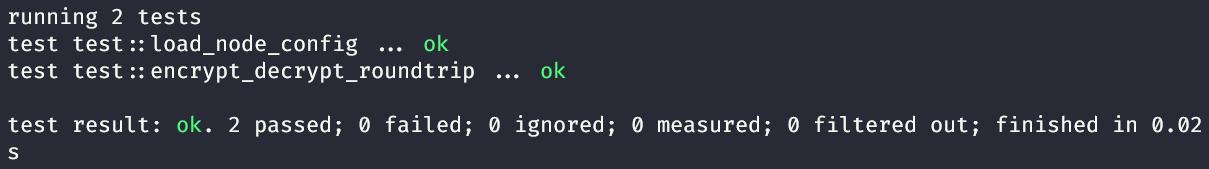
\includegraphics[width=1\textwidth]{tests_running.png}\par
\end{document}

